\section{Benchmark Results}
\label{cha:results}

In this section, we present and compare the findings from the data analysis for each targeted datastore, reporting values on a millisecond ($ms$) scale. Throughout the benchmarking runs, no CPU performance issues are observed on the client side (workload generator), ensuring that latency measurements remain unaffected by client limitations. Furthermore, the error rate consistently registers zero across all runs, confirming that every read request is successfully executed.

\paragraph*{EC2-RDS vs. Lambda-RDS}
\hyperref[fig:bar_rds_const]{Figure 5.1.1} and \hyperref[fig:bar_rds_bursty]{5.1.2} show that EC2-RDS outperforms Lambda-RDS by approximately $51\%$ under constant and $56\%$ under burst workload. EC2-RDS shows $41\%$ and $43\%$ lower standard deviation under constant and burst workload, respectively. Maximum latency values of EC2-RDS are $82\%$ and $56\%$ lower under constant and burst workload, respectively.
%
\hyperref[fig:ts_rds_const]{Figure 5.2.1} and \hyperref[fig:ts_rds_bursty]{5.2.2} show that Lambda-RDS latency often experiences abrupt increases or decreases and persists at such levels for several hours, but in contrast, EC2-RDS latency remains comparatively stable. The second runs of EC2-RDS under both workload patterns outperform the initial runs.
%
Across both runs and workloads, EC2-RDS records 962 outliers with latencies between $5ms$ and $464ms$, while Lambda-RDS records 1879 outliers, ranging from $11ms$ to $818ms$.


\paragraph*{EC2-DynamoDB vs. Lambda-DynamoDB}
\hyperref[fig:bar_ddb_const]{Figure 5.1.3} and \hyperref[fig:bar_ddb_bursty]{5.1.4} show that EC2-DynamoDB outperforms Lambda-DynamoDB by approximately $14\%$ under constant and $16\%$ under burst workload. Lambda-DynamoDB shows $21\%$ and $7\%$ lower standard deviation under constant and burst workload, respectively. Maximum latency values are identical across both pairs and modes.
%
Although Lambda-DynamoDB shows lower latency variance, \hyperref[fig:ts_ddb_const]{Figure 5.2.3} and \hyperref[fig:ts_ddb_bursty]{5.2.4} reveal that Lambda-DynamoDB exhibits sudden, temporary latency spikes under both workloads, with peaks significantly exceeding those of EC2-DynamoDB. As with EC2-RDS, the second runs of EC2-DynamoDB under both workloads outperform the initial runs, particularly during the burst workload.
%
Across both runs and workloads, EC2-DynamoDB records 3956 outliers with latencies between $7ms$ and $100ms$, while Lambda-DynamoDB records 3073 outliers, ranging from $8ms$ to $209ms$.

\paragraph*{EC2-S3 vs. Lambda-S3}
\hyperref[fig:bar_s3_const]{Figure 5.1.5} and \hyperref[fig:bar_s3_bursty]{5.1.6} show that EC2-S3 outperforms Lambda-S3 by approximately $9\%$ under both constant and burst workload. Lambda-S3 shows a $20\%$ lower standard deviation under constant but $15\%$ higher under burst workload. The maximum latency value of Lambda-S3 is $32\%$ lower under constant but $11\%$ higher under burst workload.
%
Unlike RDS and DynamoDB, \hyperref[fig:ts_s3_const]{Figure 5.2.5} and \hyperref[fig:ts_s3_bursty]{5.2.6} show that Lambda-S3 latency does not experience temporal performance shifts or large spikes. Additionally, for EC2-S3, the second runs under both workload patterns do not show better performance compared to the initial runs, a trend observed with RDS and DynamoDB.
%
Across both runs and workloads, EC2-S3 records 128 outliers with latencies between $22ms$ and $834ms$, while Lambda-S3 records 148 outliers, ranging from $26ms$ to $390ms$.

\paragraph*{Summary}
The benchmark results indicate that RDS, DynamoDB, and S3 paired with EC2 generally outperform those paired with Lambda in terms of mean latency. However, the absolute difference between EC2- and Lambda-based pair's mean latencies remains minimal, consistently under $1.34ms$ across all experiments. Standard deviation and outliers, on the other hand, do not show a consistent pattern across the pairs. 

\begin{figure}[h]
	\begin{subfigure}{0.49\linewidth}
		\centering
		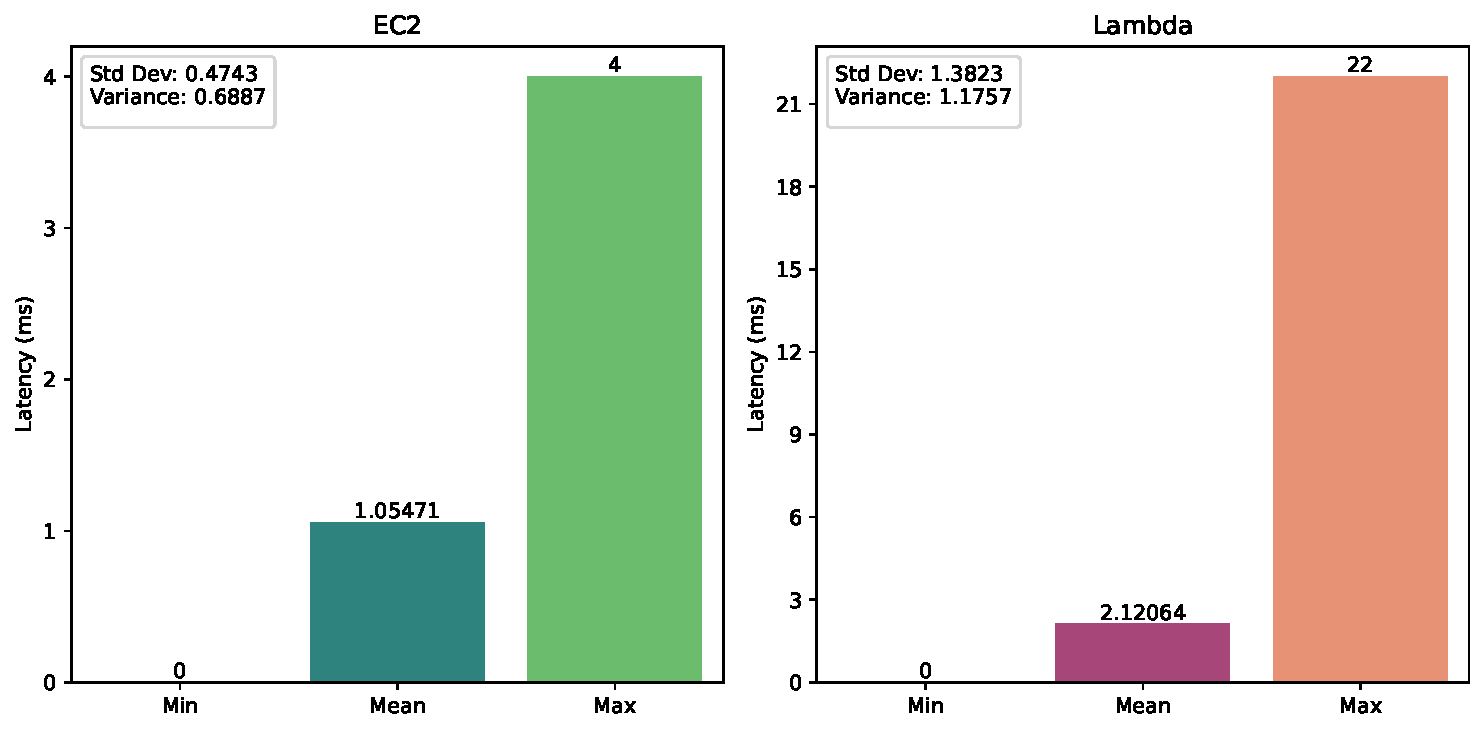
\includegraphics[width=\linewidth]{./fig/bar-rds-constant.pdf}
		\caption{Constant Workload on RDS}
		\label{fig:bar_rds_const}
	\end{subfigure}
	\hfill
	\begin{subfigure}{0.49\linewidth}
		\centering
		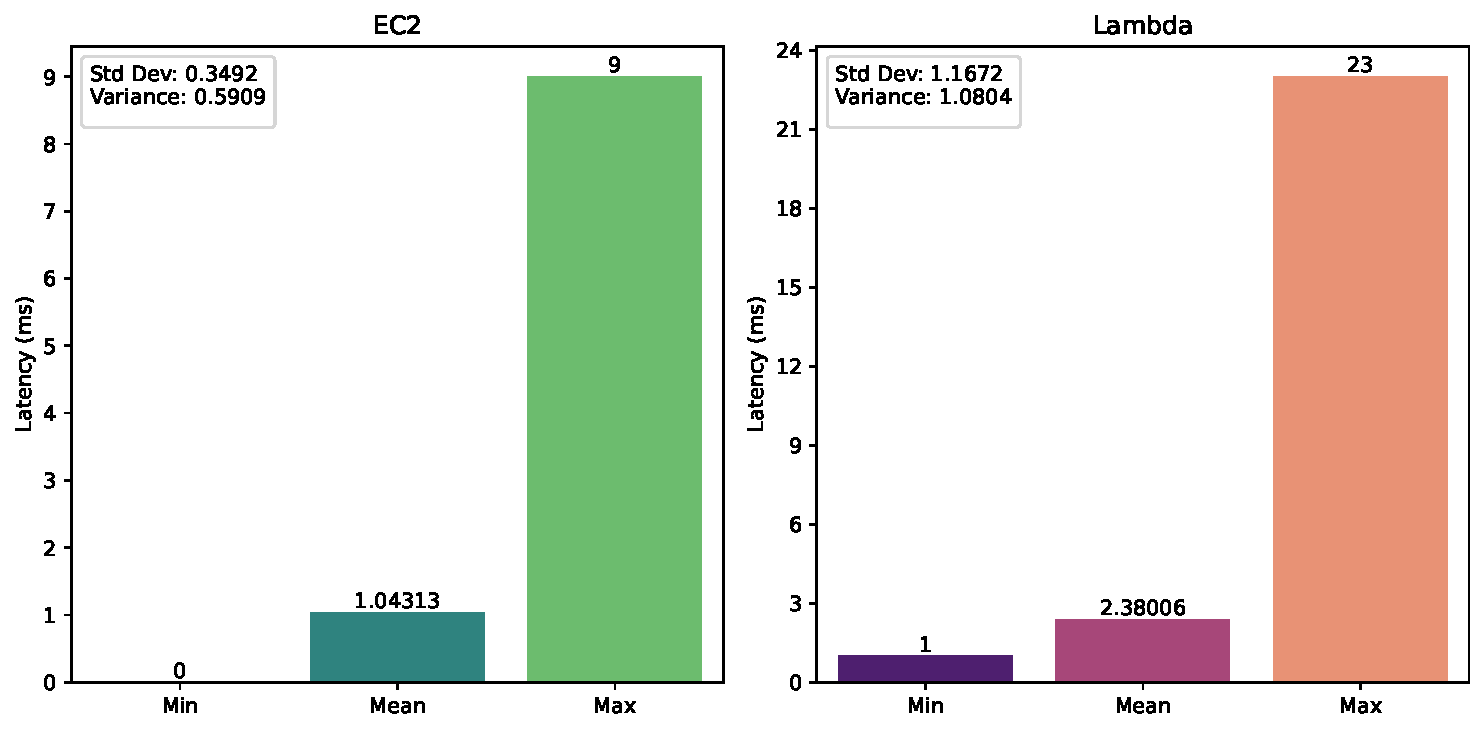
\includegraphics[width=\linewidth]{./fig/bar-rds-bursty.pdf}
		\caption{Burst Workload on RDS}
		\label{fig:bar_rds_bursty}
	\end{subfigure}
	\vfill
	\begin{subfigure}{0.49\linewidth}
		\centering
		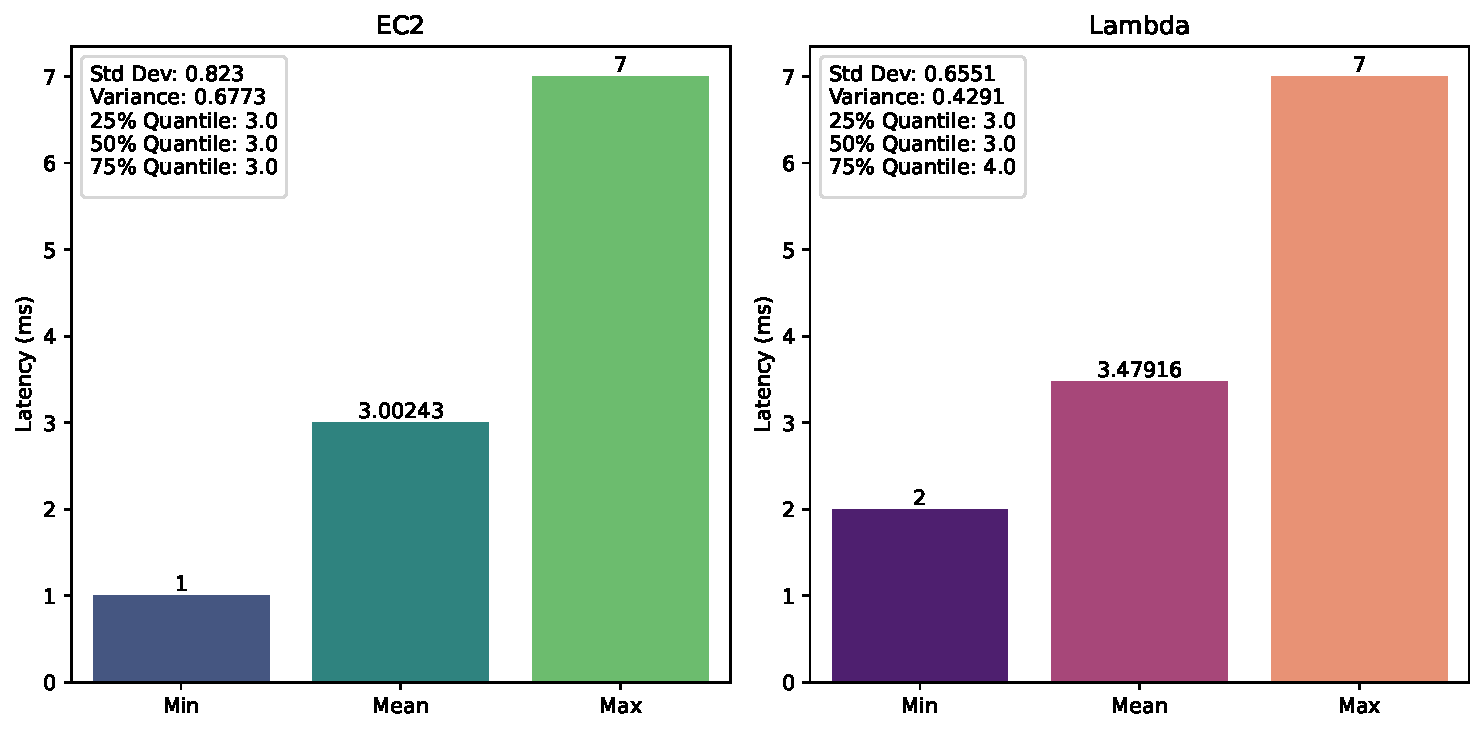
\includegraphics[width=\linewidth]{./fig/bar-dynamo-constant.pdf}
		\caption{Constant Workload on DynamoDB}
		\label{fig:bar_ddb_const}
	\end{subfigure}
	\hfill
	\begin{subfigure}{0.49\linewidth}
		\centering
		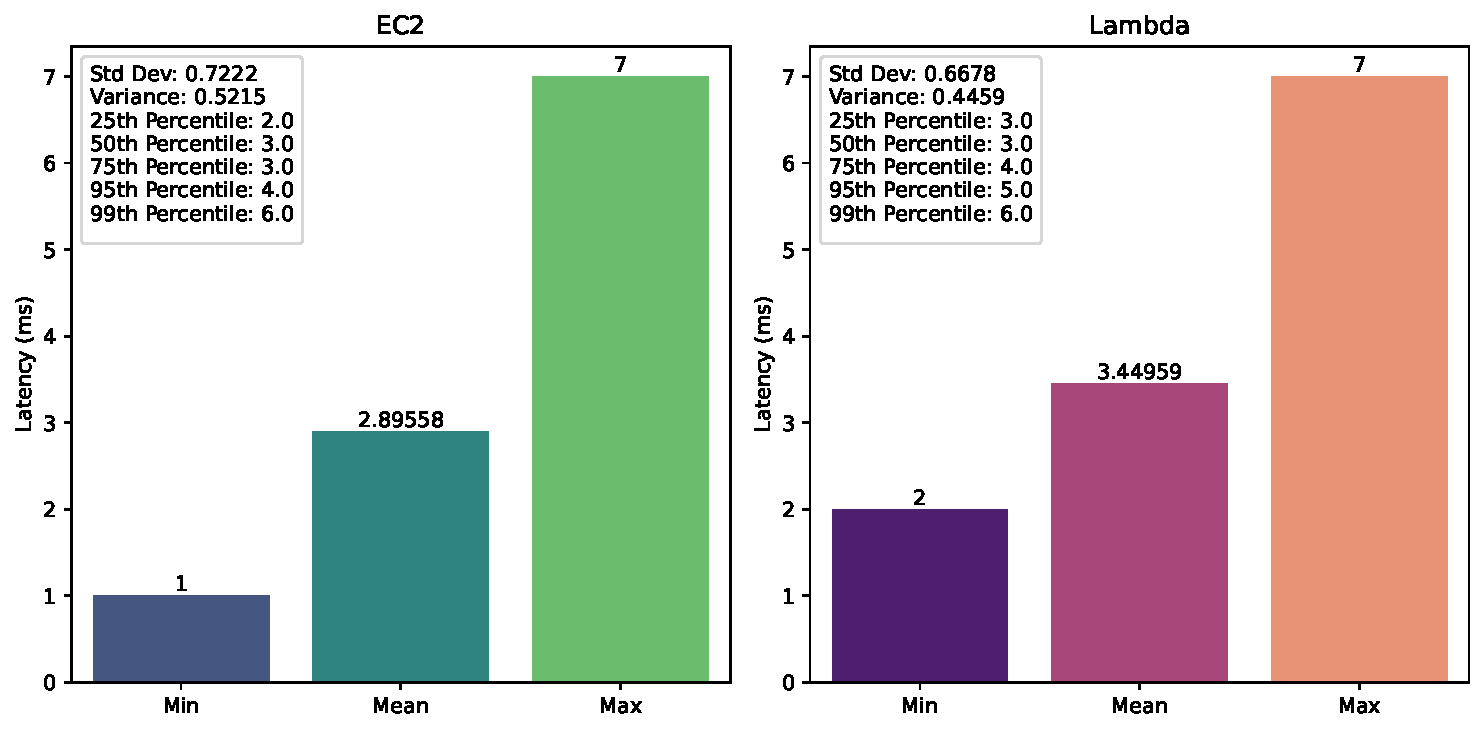
\includegraphics[width=\linewidth]{./fig/bar-dynamo-bursty.pdf}
		\caption{Burst Workload on DynamoDB}
		\label{fig:bar_ddb_bursty}
	\end{subfigure}
	\vfill
	\begin{subfigure}{0.49\linewidth}
		\centering
		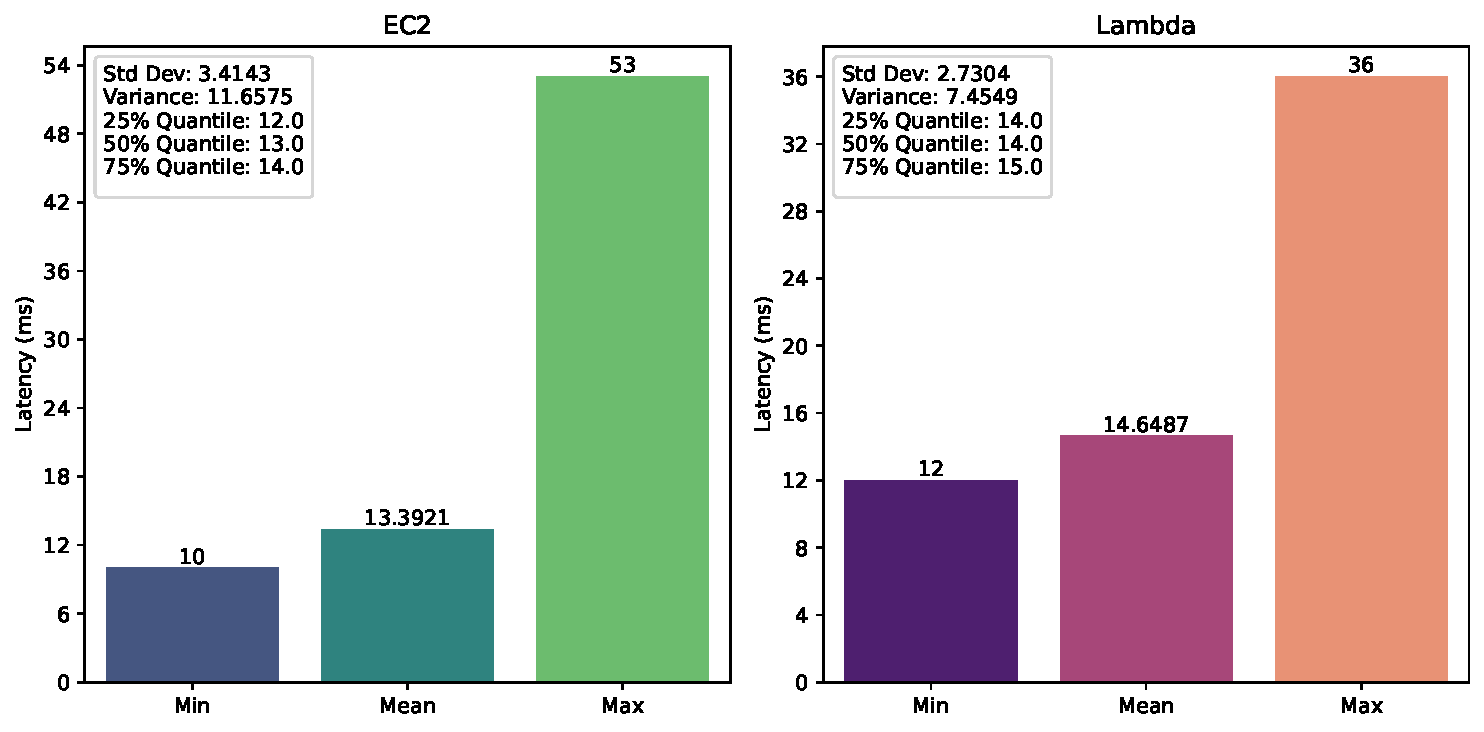
\includegraphics[width=\linewidth]{./fig/bar-s3-constant.pdf}
		\caption{Constant Workload on S3}
		\label{fig:bar_s3_const}
	\end{subfigure}
	\hfill
	\begin{subfigure}{0.49\linewidth}
		\centering
		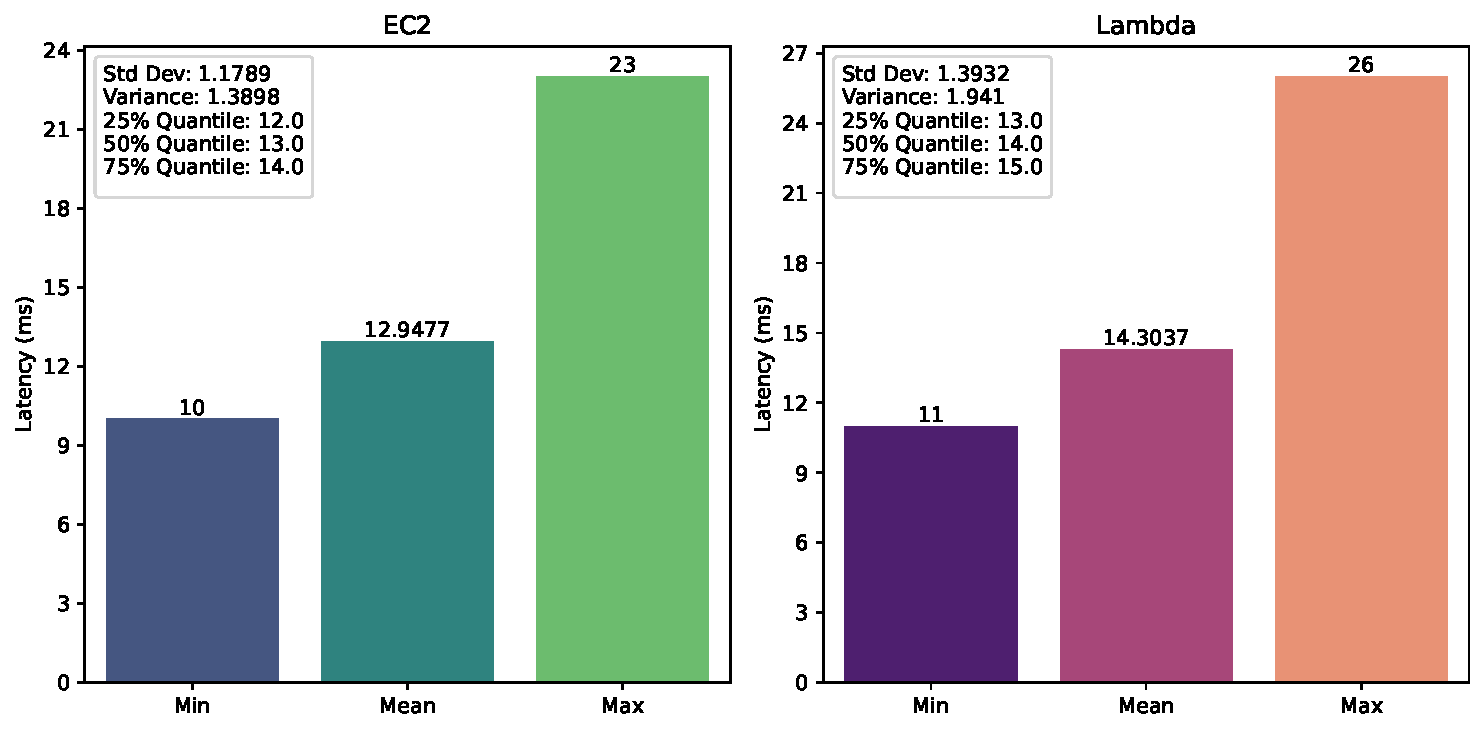
\includegraphics[width=\linewidth]{./fig/bar-s3-bursty.pdf}
		\caption{Burst Workload on S3}
		\label{fig:bar_s3_bursty}
	\end{subfigure}
	\caption{Aggregation of Latency Measurements}
	\label{fig:bar-plots}
\end{figure}

\begin{figure}[h]
	\begin{subfigure}{0.49\linewidth}
		\centering
		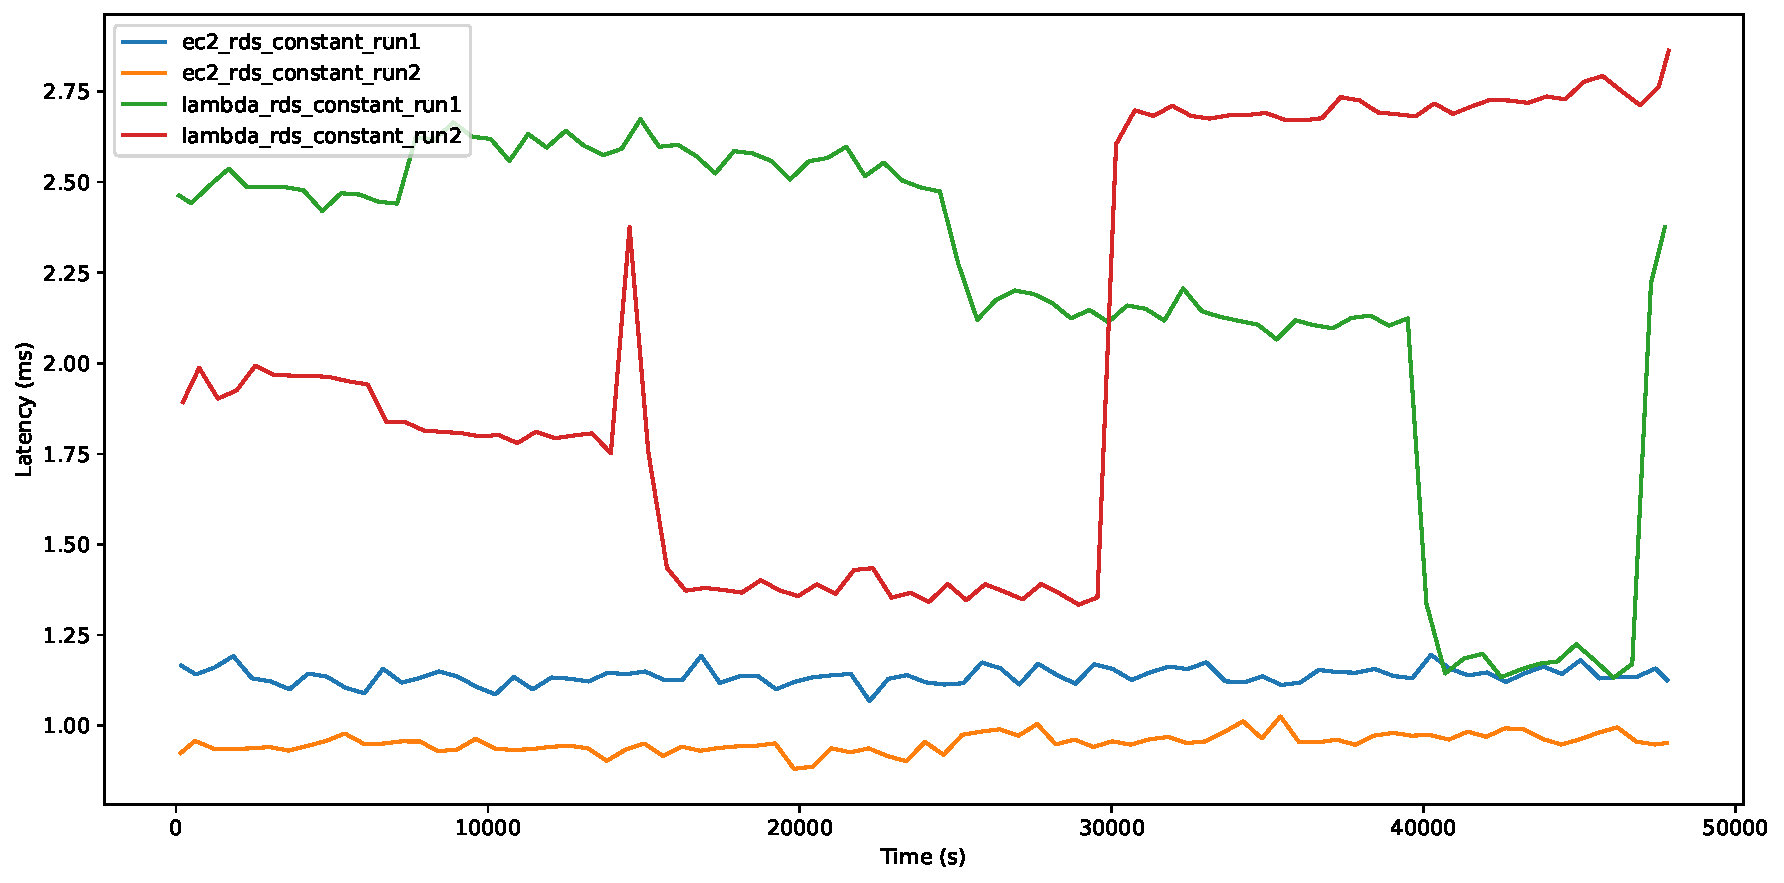
\includegraphics[width=\linewidth]{./fig/ts-rds-constant.pdf}
		\caption{Constant Workload on RDS}
		\label{fig:ts_rds_const}
	\end{subfigure}
	\hfill
	\begin{subfigure}{0.49\linewidth}
		\centering
		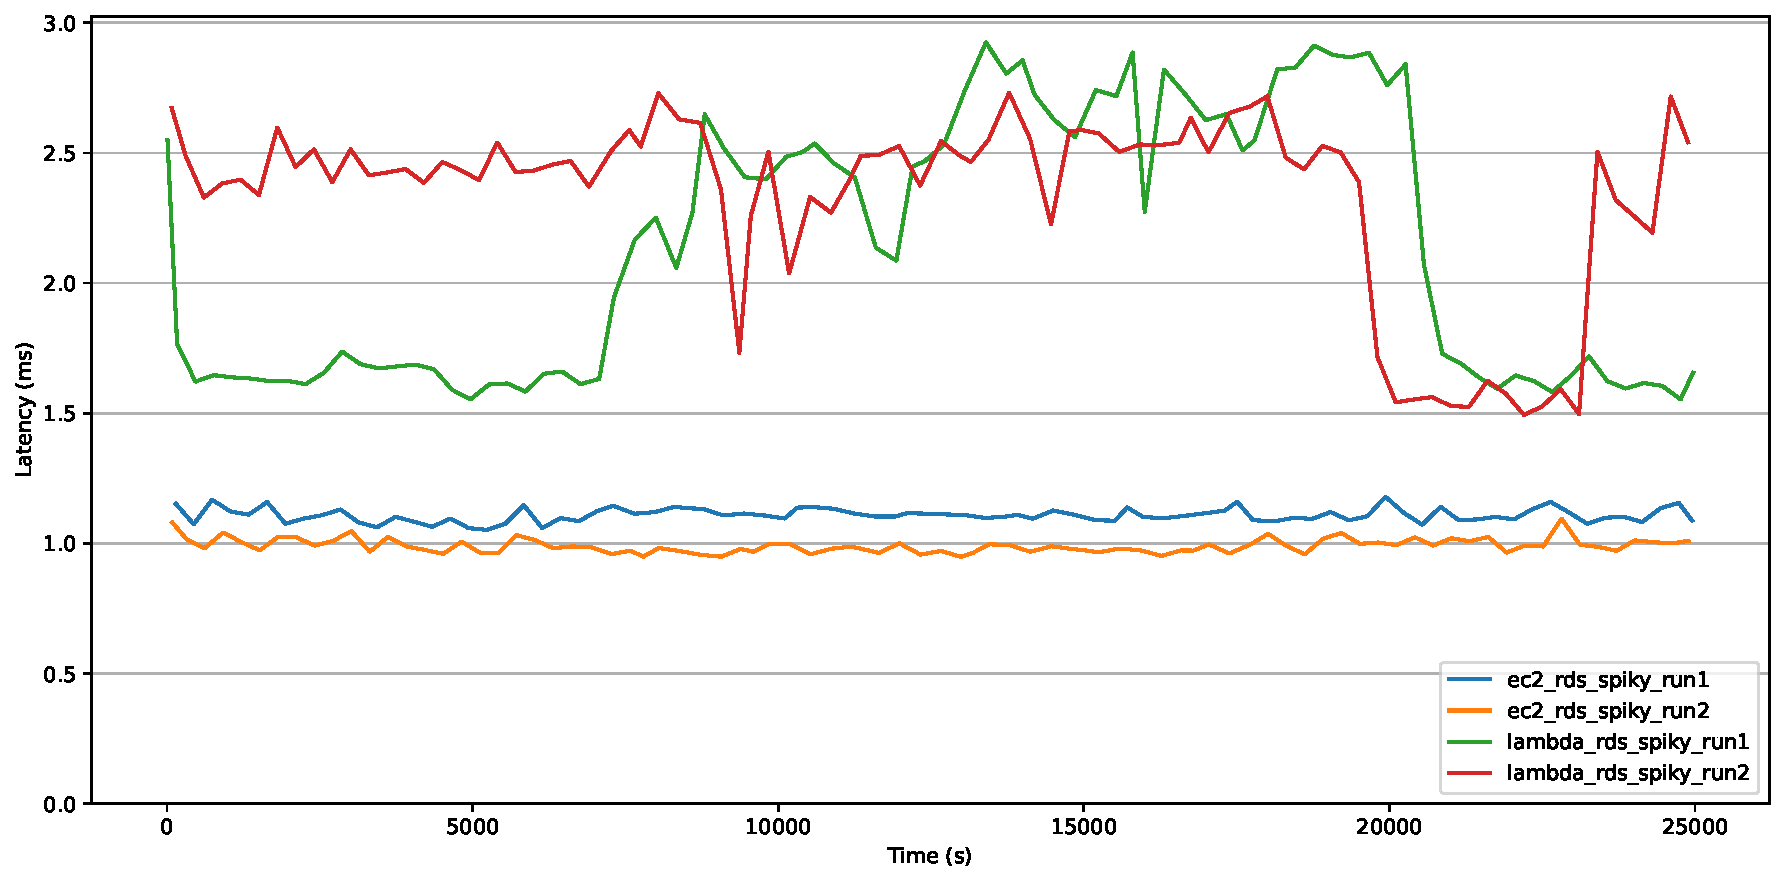
\includegraphics[width=\linewidth]{./fig/ts-rds-bursty.pdf}
		\caption{Burst Workload on RDS}
		\label{fig:ts_rds_bursty}
	\end{subfigure}
	\vfill
	\begin{subfigure}{0.49\linewidth}
		\centering
		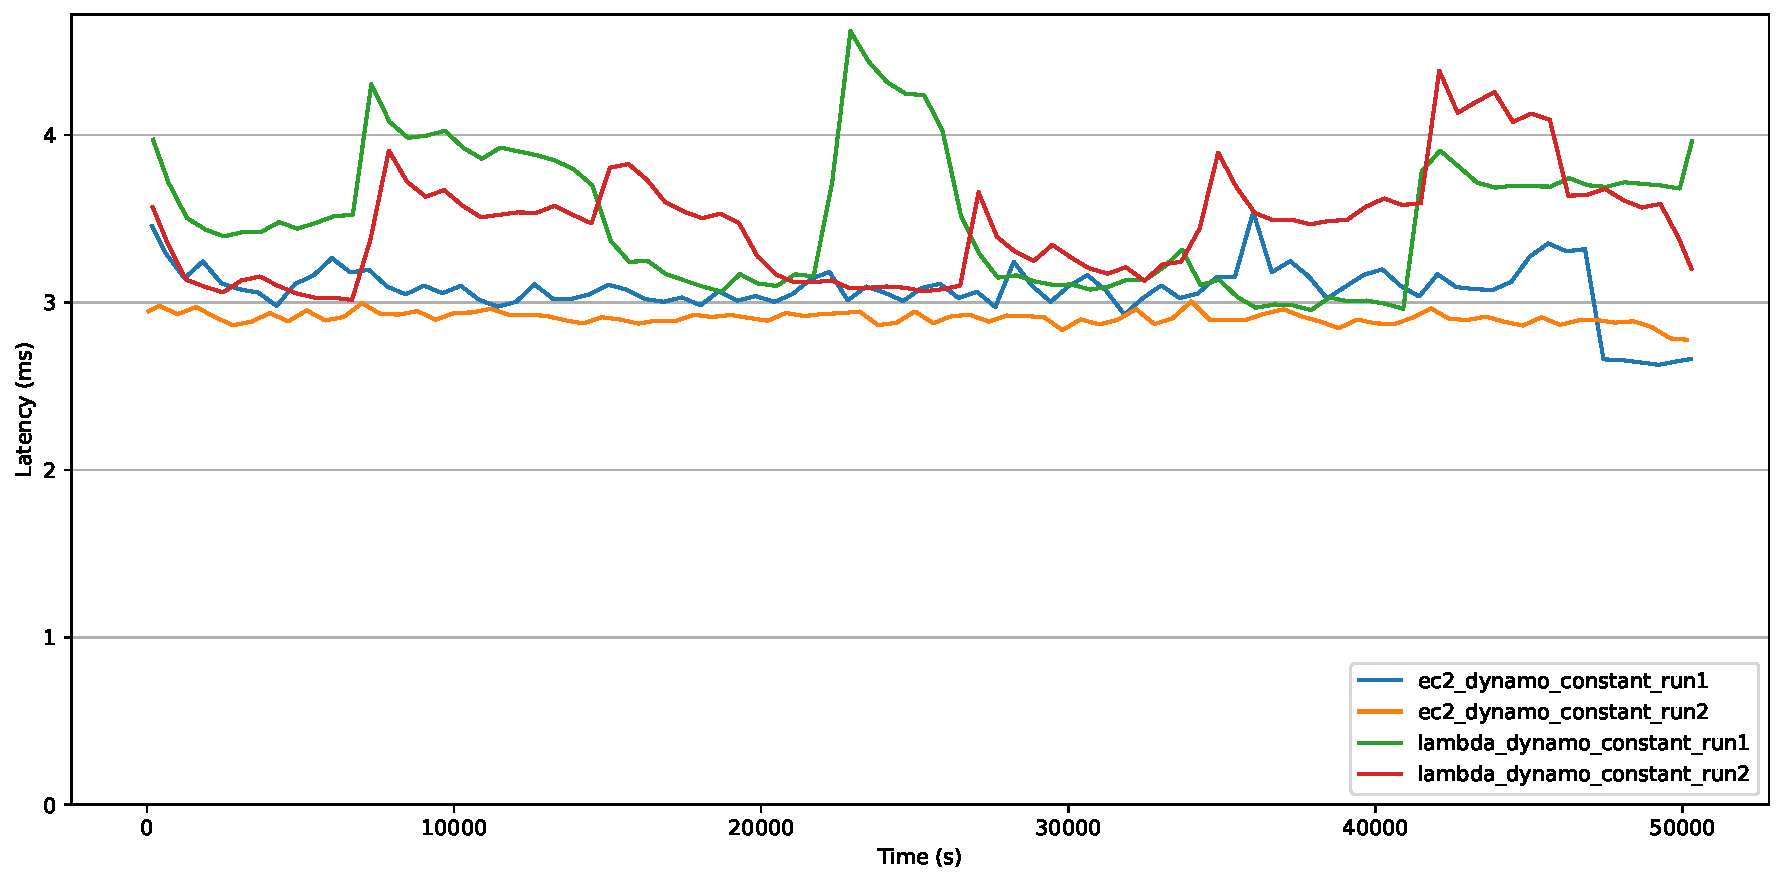
\includegraphics[width=\linewidth]{./fig/ts-dynamo-constant.pdf}
		\caption{Constant Workload on DynamoDB}
		\label{fig:ts_ddb_const}
	\end{subfigure}
	\hfill
	\begin{subfigure}{0.49\linewidth}
		\centering
		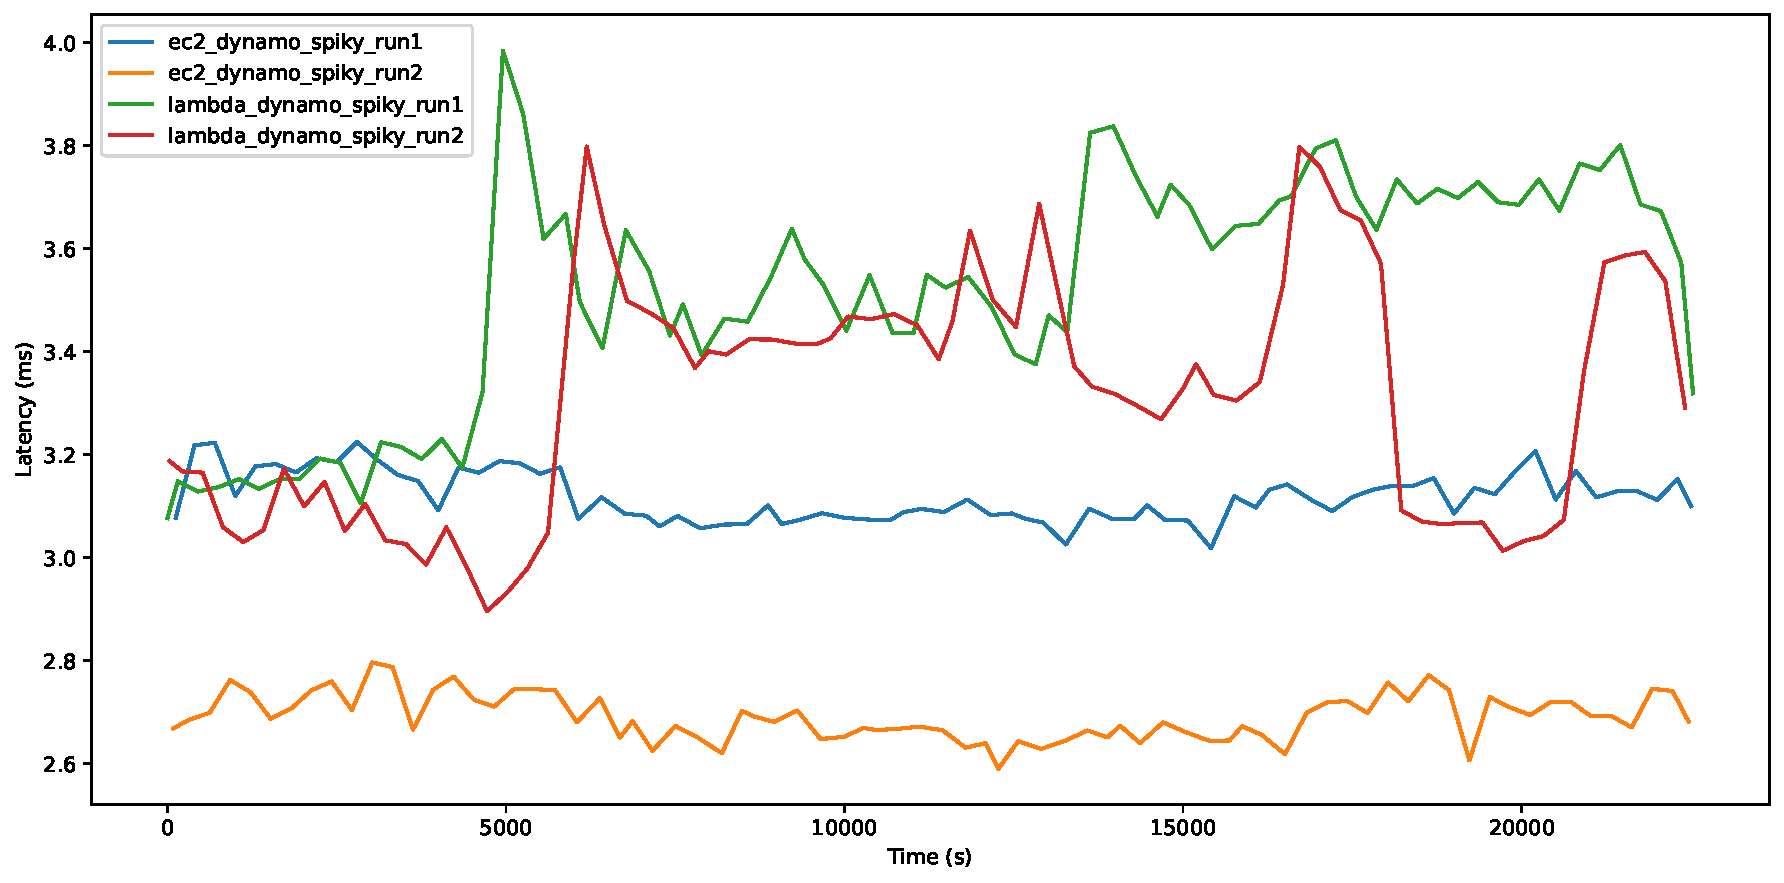
\includegraphics[width=\linewidth]{./fig/ts-dynamo-bursty.pdf}
		\caption{Burst Workload on DynamoDB}
		\label{fig:ts_ddb_bursty}
	\end{subfigure}
	\vfill
	\begin{subfigure}{0.49\linewidth}
		\centering
		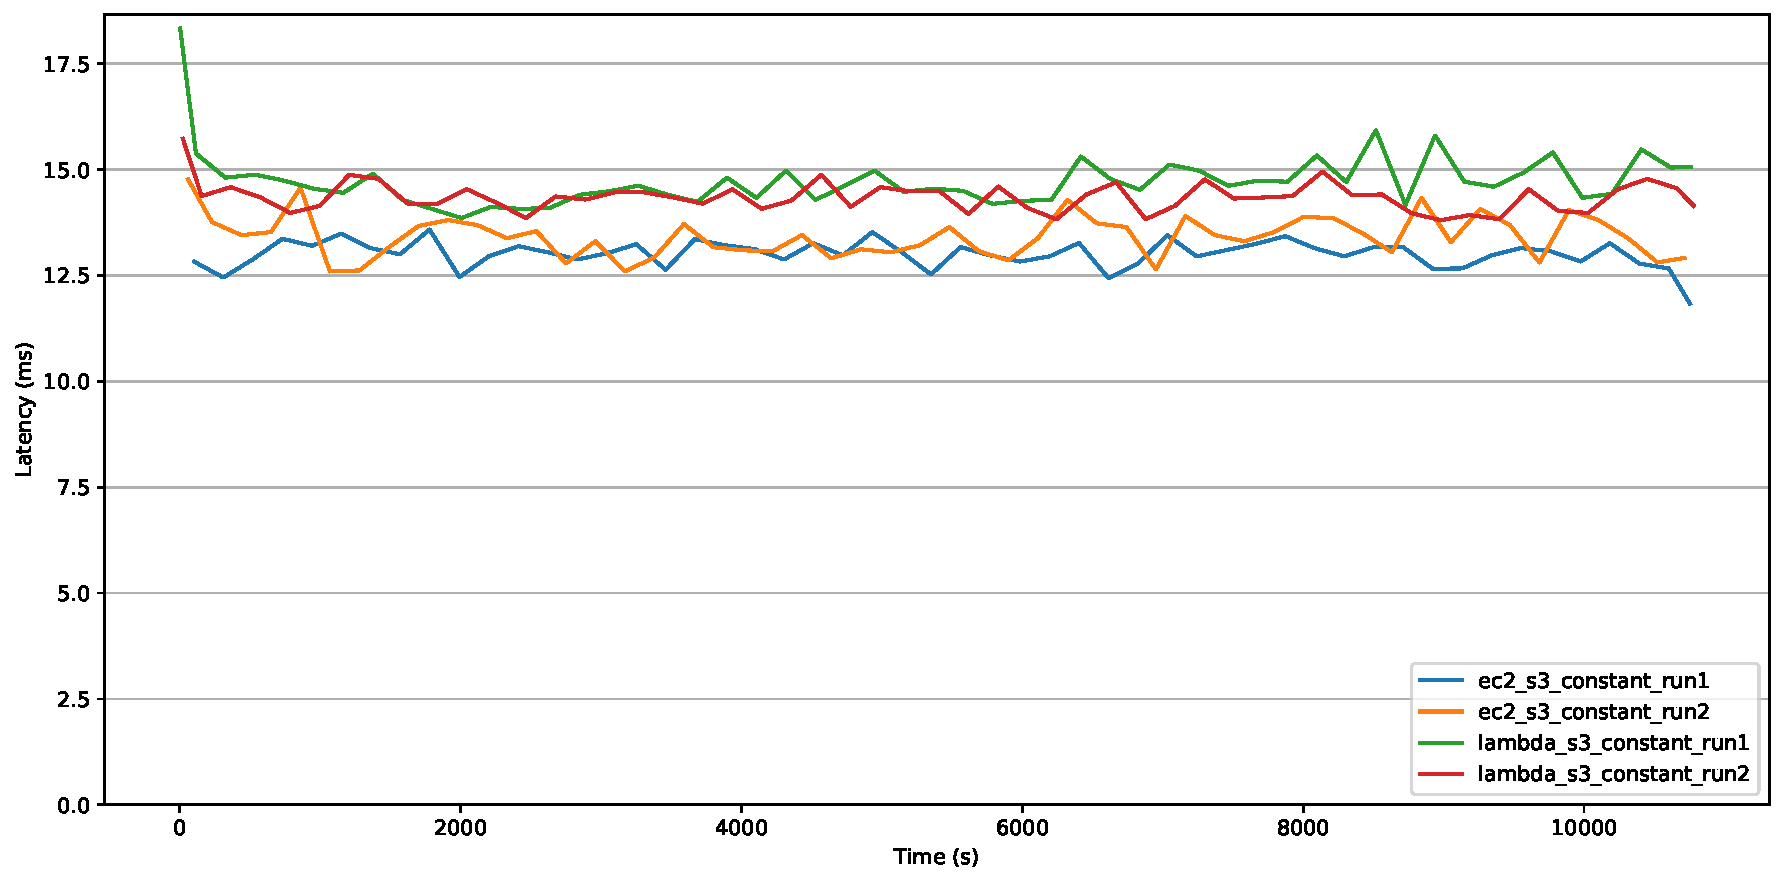
\includegraphics[width=\linewidth]{./fig/ts-s3-constant.pdf}
		\caption{Constant Workload on S3}
		\label{fig:ts_s3_const}
	\end{subfigure}
	\hfill
	\begin{subfigure}{0.49\linewidth}
		\centering
		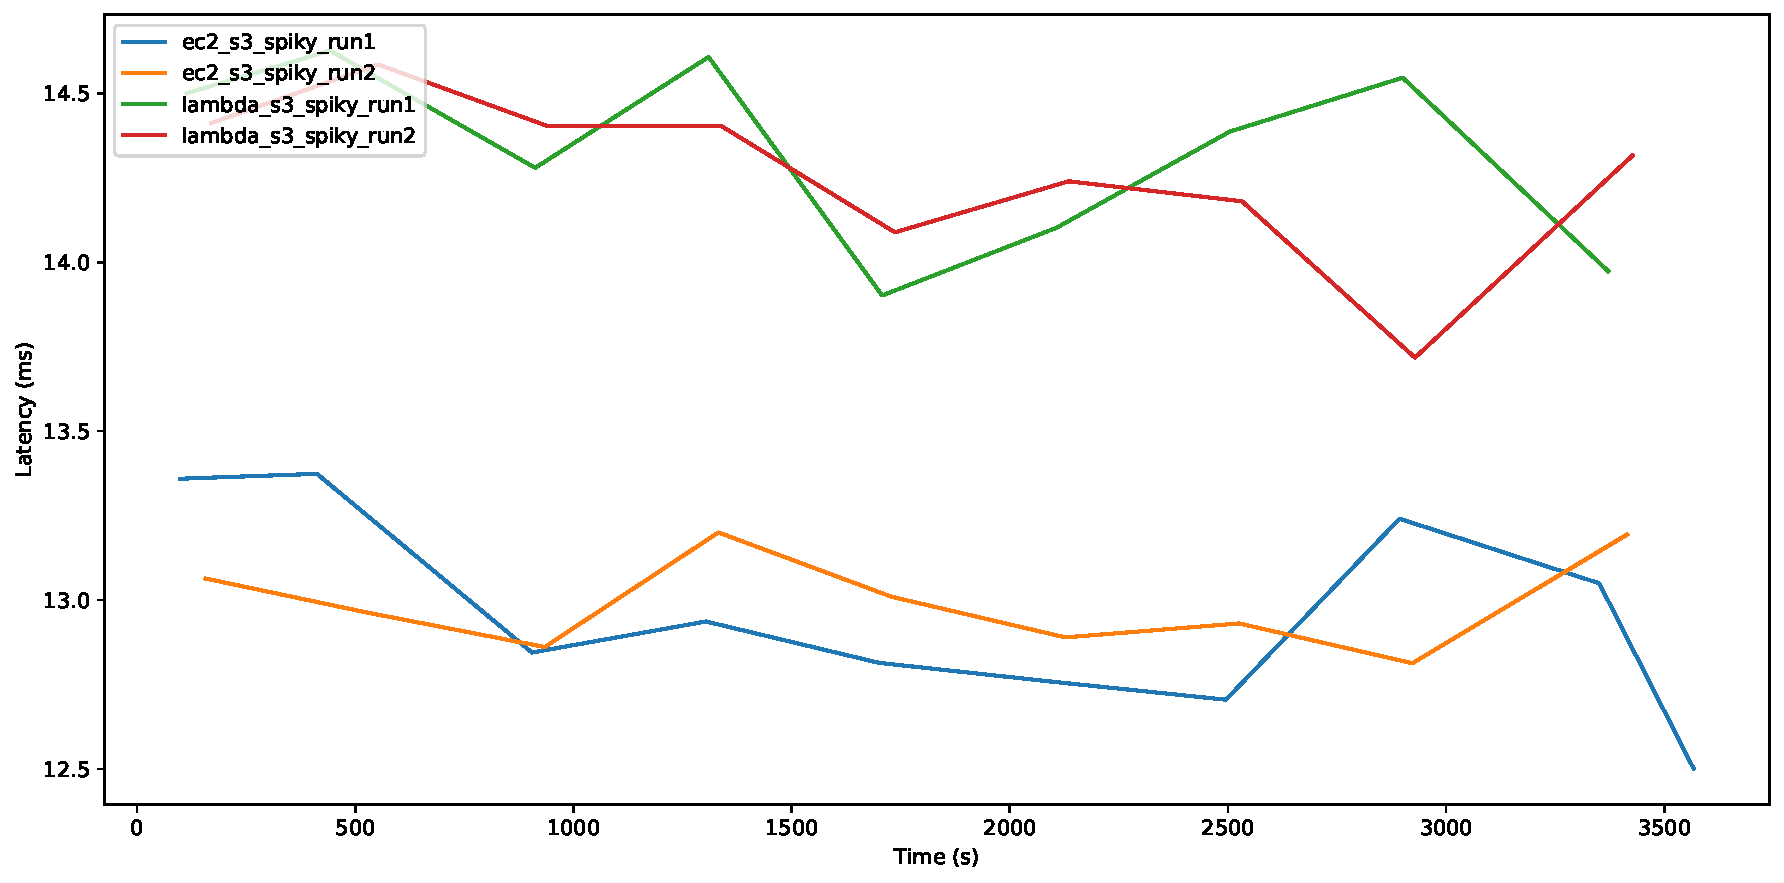
\includegraphics[width=\linewidth]{./fig/ts-s3-bursty.pdf}
		\caption{Burst Workload on S3}
		\label{fig:ts_s3_bursty}
	\end{subfigure}
	\caption{Time-Series Representation of Latency Measurements}
	\label{fig:ts-plots}
\end{figure}
